\lstset{language=Matlab}
\lstset{frame=single}
\section{Matlab}
First the SeparateColors.m function is used to filter out the different colors. It takes in a multi-color-image matrix, and returns six images. Each image contains only the non-stops of a certain color. The images are generated by subtracting the unwanted colors, and increasing the values of the wanted colors.
For example: The blue non-stops are separated by subtracting the green-image from the blue-image, thus removing green nonstops. 
\\
\centerline{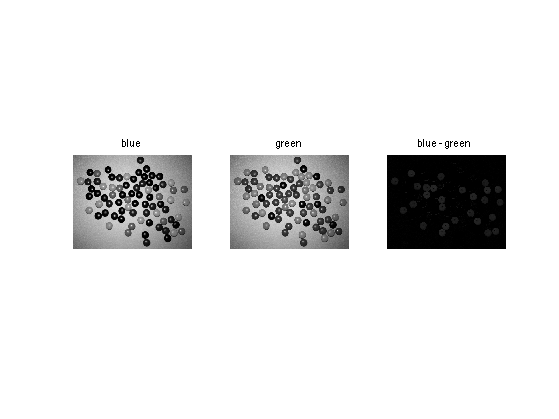
\includegraphics[clip=true, trim=40 100 40 80]{separate_step1.png}}
\\
As the green and the blue images look quite alike, the resulting image is mostly black. To be able to further subtract colors from the image, the max values are increased. Red colors are then subtracted from the image.
\\
\centerline{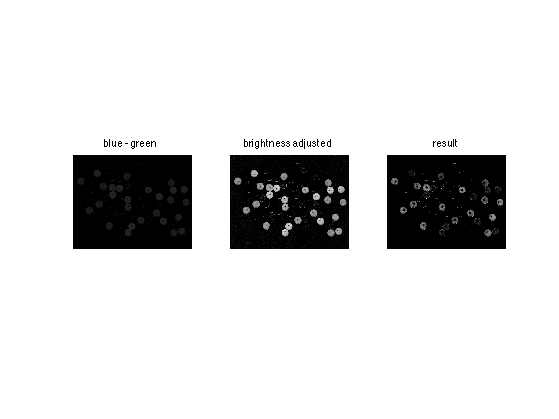
\includegraphics[clip=true, trim=40 100 40 80]{separate_step2_1.png}}
\\
Below is the code that generated the resulting image. 
\lstinputlisting[firstline=20, lastline=26]{../matlab/separateColors.m}
\\
The image created so far has the blue objects represented as the brightest circles. To remove the unwanted representation of other objects, thrsholding is used.
\\
\lstinputlisting[firstline=43, lastline=43]{../matlab/separateColors.m}
\\
To remove noise from the images, the images are median filtered. This is done by the function Median filter. 
\\
\lstinputlisting{medianFilter.m}
\\
\centerline{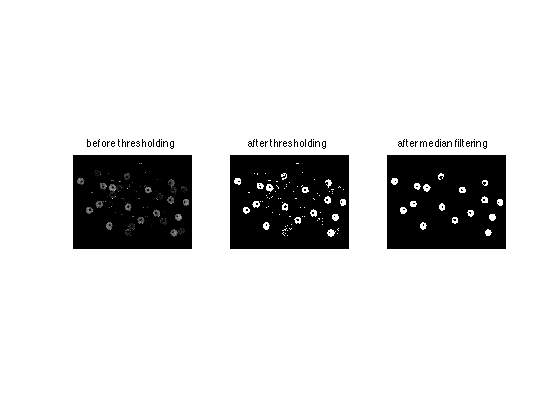
\includegraphics[clip=true, trim=40 100 40 80]{separate_step3_1.png}}
\\

\subsection{Improvements}
A more adjustable but computational heavier approach to separate colors in the image, is by filtering. Each matrix would then have to be filtered, to extract the r, g and b values. An appropriate range would have to be set, for this method to work. For example: The blue non-stops in a image would be separated by filtering the values 0 to 50 from the red matrix, 0 to 50 from the green matrix and 205 to 255 from the blue image. A new matrix is then generated. The overlapping values are represented as 1.0 in the new matrix. The remaining values are set to 0.0. 
\\



